\section{Prototype}

O padrão Prototype permite reduzir a quantidade 
de subclasses definidas em uma aplicação 
substituindo-as por instâncias predefinidas 
que podem ser especificadas em tempo de 
execução. Objetos que funcionm como 
protótipos podem ser clonados e assim 
reutilizados por outros objetos como uma 
alternativa à herança. 

A estrutura do padrão, apresentada na imagem 
\ref{prototype_struct}, mostra uma interface 
Prototype que define a operação Clone, responsável 
por copiar o protótipo reutilizável de um objeto. 
As classes ConcretePrototype implementam essa 
interface e a operação que retorna essa cópia. 
Por fim, a classe Client possui uma referência 
para um protótipo, recebida através da operação 
Clone. Essa dinâmica permite que a classe cliente 
não precise conhecer o objeto protótipo nem sua 
implementação, o que as torna independentes e 
diminui o acoplamento.

\begin{figure}[htb]
	\caption{\label{prototype_struct}Estrutura do Prototype}
	\begin{center}
	    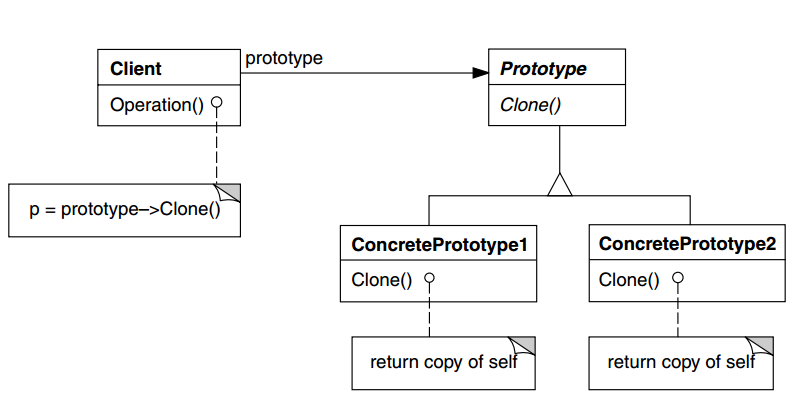
\includegraphics[scale=0.5]{5_padroes-contexto-funcional/5.1_criacionais/5.1.4_prototype/diagram.png}
	\end{center}
\end{figure}


\subsection*{Exemplo Orientado a Objetos}

Como exemplo de uso do Prototype, um 
\textit{framework} de editores gráficos deseja 
ser utilizado para construir um editor de 
partituras musicais. A classe responsável pelo 
desenho de elemntos gráficos na tela não 
conhece as classes de notas musicais que 
precisam ser desenhadas. Ao invés de criar uma 
subclasse para cada novo elemento gráfico, 
a classe responsável pelo desenho 
pode ser implementada de forma que receba 
um objeto protótipo que não precisa ser 
conhecido. Dessa forma, trocando a herança 
por uma delegação, é possível desenhar qualquer 
elemento musical, desde que ele possa ser 
clonado. A figura \ref{prototype_exemplo} e 
o código \ref{ooprototype} ilustram esse cenário.

\begin{figure}[htb]
	\caption{\label{prototype_exemplo}Exemplo de Prototype}
	\begin{center}
	    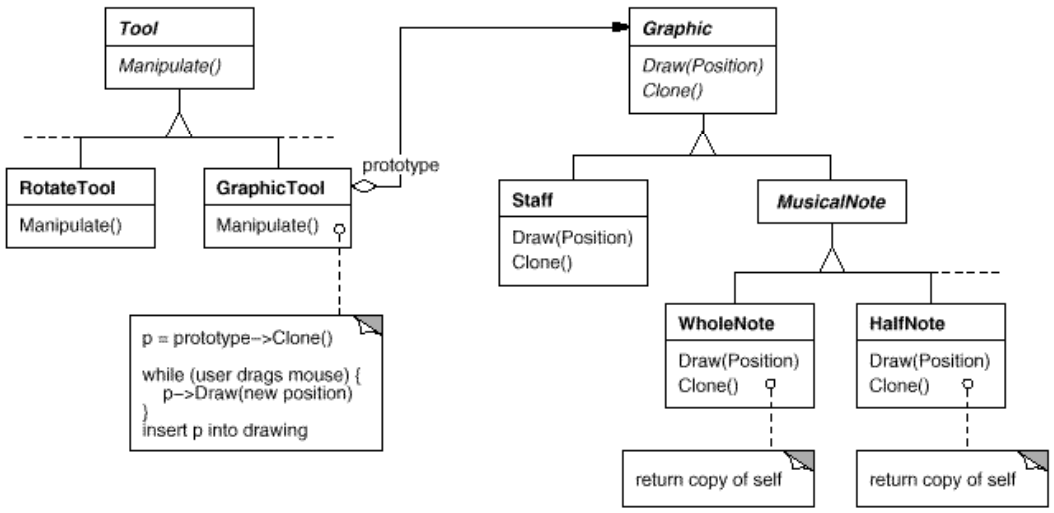
\includegraphics[scale=0.4]{5_padroes-contexto-funcional/5.1_criacionais/5.1.4_prototype/exemplo_prototype.png}
	\end{center}
\end{figure}

\begin{lstlisting}[caption={Prototype Orientado a Objetos},label=ooprototype]

trait Graphic {
	def Draw(position : Position);
	def Clone() : Graphic;
}

class Staff implements Graphic() {
	def Draw(position : Position) {
		// operação de desenho do elemento
	}

	def Clone() : Graphic {
		return this.copy();
	}
}

trait MusicalNote implements Graphic

class WholeNote implements MusicalNote() {
	def Draw(position : Position) {
		// operação de desenho do elemento
	}

	def Clone() : Graphic {
		return this.copy();
	}
}

class HalfNote implements MusicalNote() {
	def Draw(position : Position) {
		// operação de desenho do elemento
	}
	
	def Clone() : Graphic {
		return this.copy();
	}
}

class GraphicTool() {

	val prototype : Graphic;

	def Manipulate() {
		
	p = prototype.Clone();

		while(user.DragsMouse()){
			p.Draw(newPosition)
		}

		// ...
	}


}

\end{lstlisting}

\subsection*{Contexto Funcional}


\begin{lstlisting}[caption={Prototype Funcional},label=fpprototype]
    

    
\end{lstlisting}